\documentclass[border=4pt]{standalone}
% Preámbulo común de las figuras. Cada figura es un documento standalone
% que se compila a SVG con scripts/build_figures.sh
\usepackage[utf8]{inputenc}
\usepackage{amsmath}
\usepackage{tikz}
\usepackage[american, siunitx]{circuitikz}
\usetikzlibrary{arrows.meta,calc,decorations.pathmorphing,patterns}
\tikzset{
  >={Stealth[length=2.2mm]},
  eje/.style={->, thin},
  hilo/.style={thick},
}
% Paleta común: tonos medios legibles sobre fondo claro
\definecolor{azul}{RGB}{31,94,168}
\definecolor{rojo}{RGB}{192,57,43}
\definecolor{verde}{RGB}{39,128,73}
\definecolor{naranja}{RGB}{211,120,30}
\definecolor{morado}{RGB}{125,60,152}

\begin{document}
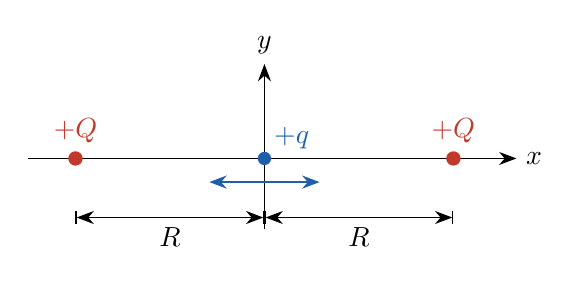
\begin{tikzpicture}[scale=1.0]
  \draw[eje] (-3.0,0) -- (3.2,0) node[right]{$x$};
  \draw[eje] (0,-0.9) -- (0,1.2) node[above]{$y$};
  \fill[rojo] (-2.4,0) circle (2.6pt) node[above=2pt]{$+Q$};
  \fill[rojo] (2.4,0) circle (2.6pt) node[above=2pt]{$+Q$};
  \fill[azul] (0,0) circle (2.4pt) node[above right]{$+q$};
  \draw[<->, thick, azul] (-0.7,-0.3) -- (0.7,-0.3);
  \draw[|<->|] (-2.4,-0.75) -- node[below]{$R$} (0,-0.75);
  \draw[|<->|] (0,-0.75) -- node[below]{$R$} (2.4,-0.75);
\end{tikzpicture}
\end{document}
